\documentclass{bioinfo}
\copyrightyear{2015}
\pubyear{2015}

\begin{document}
\firstpage{1}

\title[ChIP-seq joint discretization with quality control]{Zerone: a ChIP-seq
discretizer for multiple replicates with built-in quality control}
\author[Cusc\'o \textit{et~al}]{Pol Cusc\'o\,$^{1,2}$ and Guillaume
Filion\,$^{1,2}$\footnote{to whom correspondence should be addressed}}
\address{$^{1}$Genome Architecture, Gene Regulation, Stem Cells and Cancer
Programme, Centre for Genomic Regulation (CRG), Dr. Aiguader 88, 08003
Barcelona, Spain.\\
$^{2}$Universitat Pompeu Fabra (UPF), Barcelona, Spain.}

\history{Received on XXXXX; revised on XXXXX; accepted on XXXXX}

\editor{Associate Editor: XXXXXXX}

\maketitle

\begin{abstract} % max 150 words recommended

\section{Motivation:}
Chromatin immunoprecipitation followed by high-throughput sequencing (ChIP-seq)
is the standard method to investigate chromatin protein composition. As the
number of community-available ChIP-seq profiles increases, it becomes more
common to use data from different sources, which makes joint analysis
challenging. Issues such as lack of reproducibility, heterogeneous quality and
conflicts between replicates become evident when comparing datasets, especially
when they are produced by different laboratories.

\section{Results:}
Here we present Zerone, a ChIP-seq discretizer with built-in quality control.
Zerone is powered by a Hidden Markov Model (HMM) with zero-inflated negative
multinomial emissions, which allows it to merge several replicates into a single
discretized profile. To identify low quality or irreproducible data, we trained
a Support Vector Machine (SVM) and integrated it as part of the discretization
process. Zerone identified low quality data with 95\% accuracy. In terms of
performance, Zerone is approximately 5 times faster than MACS for a similar
accuracy.

\section{Availability:}
Zerone is available as a command line tool and as an R package. The C
source code and R scripts can be downloaded from
\href{https://github.com/gui11aume/jahmm}{https://github.com/gui11aume/jahmm}.

\section{Contact:}
\href{guillaume.filion@gmail.com}{guillaume.filion@gmail.com}
\end{abstract}

\section{Introduction}
One of the major challenges of biology is to understand how transcription
factors and chromatin proteins coordinate genome-dependent processes
such as transcription, replication and repair. Massive research efforts
are invested into collecting protein-genome interaction data in order
to gain insight into the organization of the genome as a whole. Chromatin
immunoprecipitation followed by high throughput sequencing (ChIP-seq)
emerged as the standard method to identify the targets of a transcription
factor or a histone modification in a cell population. However, ChIP is not
fully understood and artifacts are still discovered more than 10 years after
its adoption \citep{pmid24349523, pmid24173036}. Besides, the constant
improvement of sequencing technologies makes analysis of ChIP-seq profiles
difficult to standardize. There is thus a continuous need to develop and
improve computational tools to analyse ChIP-seq data.

One of the most common analyses performed on ChIP-seq profiles is to
discretize the signal, \textit{i.e.} make calls whether the feature is
present or absent for every \textit{locus} of the genome. This may seem
dubious at first glance because the biological reality is intrinsically
quantitative, but there are several good reasons to discretize ChIP-seq
profiles: it makes the signal simpler to interpret from the human
perspective, it simplifies downstream analyses and it allows to compare or
combine profiles of different nature. This raises a challenge at the
computational level because discretization has to be carried out uniformly
for signals that may have very different properties. For instance compare
the begabase scale domains of Lamin \citep{pmid18463634} to the 6~bp
binding sites of typical transcription factors.

Large consortia such as ENCODE have brought to light a more severe type
of issue related to the quality of ChIP-seq data. Conflicts between
replicates are common, and
sometimes laboratory effects are clearly detectable in the data,
even when experimentalists use the same material and follow the same
protocol (our unpublished observations). The most popular remedy is to
use a metric called IDR (Irreproducible Discovery Rate \cite{li2011}),
which allows to weed
out poorly reproducible signal. This approach is a significant step
forward, but the IDR is undefined when more than two replicates are
available. Besides, keeping only the reproducible ChIP peaks is not
always the best option, as when one of the replicates has very low quality
for instance. In summary, how to integrate ChIP-seq data from different
sources and with variable qualities is still an open problem.

%\section{Approach}
Here we propose an approach to discretize ChIP-seq data where conflict
resolution and quality control are integrated in a tool that we called
Zerone. The key idea of Zerone is to combine an arbitrary number of
ChIP-seq replicates in a single discretized profile, where conflicts are
resolved by maximizing the likelihood of the underlying statistical model.
Following discretization, Zerone controls the quality of its output in
order to detect potential anomalies, and when applicable rejects the
output as a whole. Internally, the first step implements a Hidden Markov
Model (HMM) with zero-inflated negative multinomial (ZINM) emissions, and
the second implements a Support Vector Machine (SVM) trained using ENCODE
ChIP-seq data. HMM-based discretization is agnostic to the shape of the
signal (broad or peaky) and the ZINM distribution captures the essential
features of the read count distribution in ChIP-seq data. These two
properties provide a unified framework to discretize ChIP-seq data of
different kinds.

Zerone is designed for large volume pipelines aiming to combine many
ChIP-seq profiles with little human intervention. To this end, it is
compatible with the standard SAM and BAM formats \citep{pmid19505943},
it produces congruent window-based outputs, and it can process hundreds
of experiments per day on average hardware. We benchmarked Zerone against
MACS \citep{pmid18798982}, BayesPeak \citep{pmid19772557} and
JAMM \citep{pmid25223640} on the core
task of discretizing ChIP-seq profiles of CTCF, Pol2 and H3K36me3. Our
results show that Zerone is competitive in terms of speed and accuracy.

\begin{methods}
\section{Methods}

\subsection{Datasets and preprocessing}
We used all the ChIP-seq profiles produced by the ENCODE consortium on the human
myelogenous leukemia cell line K562. We did not make use of preprocessed mapped
reads because they could have been mapped with different software and could
therefore disagree on its results \citep{pmid21059603}. Instead, we mapped all
the raw reads onto the hg19 assembly of the human genome with GEM
\citep{pmid23103880}, using the options \texttt{--unique-mapping} and
\texttt{-q ignore} of gem-mapper, version 1.376 (beta). The version of
gem-indexer was 1.423 (beta). We preprocessed the data in the same
way both for training the classifier and for benchmarking.

For training the classifier, we binned the mapped reads into 300~bp windows and
saved the data in WIG format before discretization.

For comparing Zerone against other discretizers, we analysed three different
ChIP-seq datasets: CCCTC-binding factor (CTCF), tri-methylated histone H3 at
lysine 36 (H3K36me3) and RNA polymerase II (Pol2)---that represent punctate,
broad and mixed type signals respectively.

\subsection{Emission model}
It is natural to model read counts in genomic windows by an unbounded
discrete distribution. The Poisson distribution is an obvious candidate,
but it is a poor choice because the variance of read counts is typically
higher than the mean in ChIP-seq data. The reason is that windows are non
homogeneous, which increases the dispersion. More specifically, windows
are not equally PCR-prone and not equally mappable. The negative binomial
(NB) distribution is thus a better choice because it allows some variation
between windows. However, genomes are fraught with repeats, which creates
an excess of windows where reads cannot be mapped. Since such windows
will always have 0 read count, a natural choice for this distribution is
the zero-inflated negative binomial (ZINB), \textit{i.e.} the mixture of
a negative binomial distribution and a distribution concentrated at 0.

The ZINB distribution has 3 parameters that can be fitted by maximum
likelihood. Zerone uses a custom solver based on the Newton-Raphson
method, which converges much faster than the popular routine
\texttt{zeroinfl} \citep{psclb} from the R \citep{R} package \texttt{pscl}
\citep{pscla}.
Fig.~\ref{fig:ZINB_fit} shows that the ZINB distribution gives a better
fit to ChIP-seq data than Poisson and NB distributions.

\begin{figure}[!tpb]
\centerline{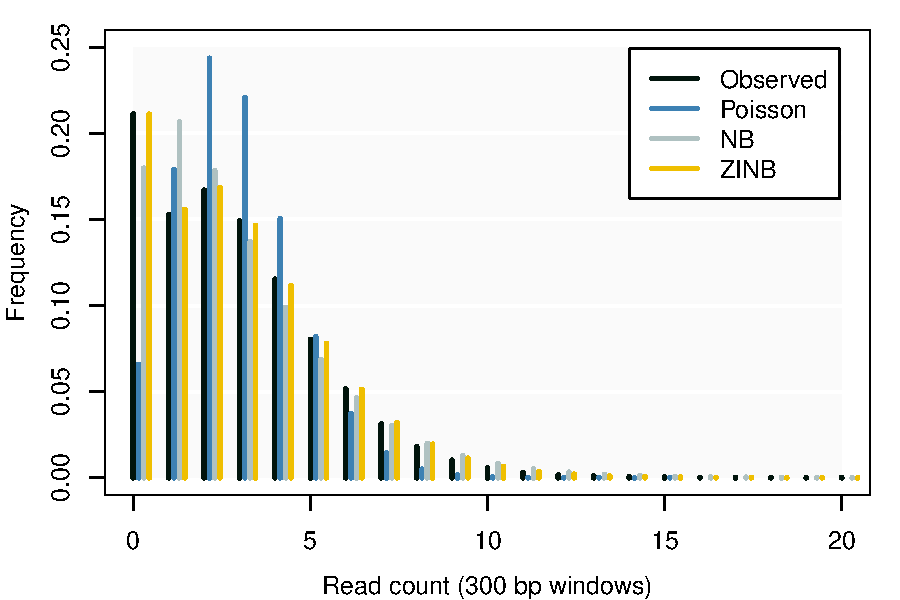
\includegraphics[scale=0.55]{ZINB_fit.pdf}}
% XX is wgEncodeSydhTfbsK562InputRawData.bed.gz %
\caption{Using the ZINB distribution to model ChIP-seq data. Reads from
the negative control dataset XX were mapped on the human genome and pooled
in 300~bp windows after removing duplicates. The histogram of the read
counts is shown in black (no immunoprecipitation was performed in this
experiment, so this variation corresponds to the `baseline'). The
histograms in gray scales show the maximum likelihood fit of the Poisson,
Negative Binomial (NB) and Zero-Inflated Negative Binomial (ZINB)
distributions. The fit of the Poisson distribution (light gray) is poor.
The NB distribution (medium gray) gives a good fit at the tail, but not
for windows with 0 and 1 read. The ZINB distribution (dark gray) gives
a good fit over the whole range.
}\label{fig:ZINB_fit}
\end{figure}

The NB distribution can be interpreted as a Gamma-Poisson process,
which gives a straightforward extension to a multivariate
distribution called the Negative Multinomial (NM) and to its
corresponding zero-inflated version the Zero-Inflated Negative
Multinomial (ZINM, see supplementary material for detail). In this model,
windows have an intrinsic ChIP-seq bias due to their G+C content,
mappability and other inherent properties, which gives a baseline
variation present in all ChIP-seq experiments performed in the same
conditions. All the replicates of a ChIP-seq experiment can thus be
combined with the negative controls in a single multivariate distribution
with a number of paramters equal to $r+2$, where $r$ is the number of
experiments.

\subsection{Classifier training}
After the analysis, Zerone returns information about the learned model, such as
the estimated transition matrix, Viterbi path, and phi and p matrices. These
features differ depending on the quality of the discretization and therefore we
used them for training a SVM \citep{Chang2011,e1071}.

We built a dataset composed of 91 positive and 53 negative manually selected
discretizations that the classifier should accept or discard, respectively.
For these positive and negative examples, we discretized experimental replicates
together with their respective input control, and subsequently decided whether
the discretizations were correct based on literature about the studied proteins.
We also included in the dataset a number of aberrant negative examples obtained
by discretizing false replicates (\textit{i.e.} profiles that were not
replicates from one another but came from two different proteins, and should
therefore disagree on which were the enriched \textit{loci}) and flat profiles
(\textit{i.e.} input profiles that were passed to Zerone as target profiles and
should not contain real enrichments at all).

We trained the SVM and selected the hyperparameters that maximized the
prediction performance on test sets using a 10-fold cross-validation scheme. We
then implemented a prediction function in Zerone that used the model trained by
the SVM to classify the discretizations and suggest whether they could be
accepted or should be discarded.

% RESULTS: Performance on test sets (around 95% on 10-fold cross-validation)
% RESULTS:  describe the shapes of the data???
% Implementation of prediction function inside Zerone

\subsection{Benchmark conditions}
We chose to include MACS because it is the \textit{de facto} standard method
for ChIP-seq peak calling; BayesPeak because, as Zerone,
it also makes use of a HMM with ZINM emissions to estimate the regions of
enrichment; and JAMM because it can perform joint analysis on experimental
replicates.

All the tests were performed on a 8-core Intel Xeon E5606 machine with 48~GB of
DDR3-RAM at 1333~MHz.

\end{methods}

\section{Results}

% give an example where using Zerone highlighted inconsistencies in published
% ChIP-seq ENCODE data, allowing us to detect noisy and non-replicating profiles
% that should be flagged as such.

\subsection{Benchmark}
%Table \ref{Tab:perf} summarize the performace results of the analyses.

%\begin{table}[!t]
%\processtable{Performance comparison between discretizers.
%\label{Tab:perf}}
%{\begin{tabular}{lll}\toprule
%\bf{Software} & \bf{Version} & \bf{Time spent (s)} \\\midrule
%BayesPeak & 1.20.0 & row1 \\
%JAMM & 1.0.7 & row2 \\
%MACS & 2.1.0 & row3 \\ %MACS callpeak
%Zerone & 1.0 & row4 \\\botrule
%\end{tabular}}{Footnote}
%\end{table}

\section{Discussion and conclusion}

\section*{Acknowledgement}

\paragraph{Funding\textcolon}
P.C. fellowship is partly financed by the Spanish Ministry of Economy and
Competitiveness (State Training Subprogram: predoctoral fellowships for the
training of PhD students (FPI) 2013).

\bibliographystyle{natbib}
\bibliography{document,extra}

\end{document}

%\begin{equation}
%\label{eq:01}
%\sum x+ y =Z
%\end{equation}

%\begin{enumerate}
%\item this is item, use enumerate
%\item this is item, use enumerate
%\item this is item, use enumerate
%\end{enumerate}

%\begin{itemize}
%\item for bulleted list, use itemize
%\item for bulleted list, use itemize
%\item for bulleted list, use itemize
%\end{itemize}

%\begin{table}[!t]
%\processtable{This is table caption\label{Tab:01}}
%{\begin{tabular}{llll}\toprule
%head1 & head2 & head3 & head4\\\midrule
%row1 & row1 & row1 & row1\\
%row2 & row2 & row2 & row2\\
%row3 & row3 & row3 & row3\\
%row4 & row4 & row4 & row4\\\botrule
%\end{tabular}}{This is a footnote}
%\end{table}

%\begin{figure}[!tpb]%figure1
%%\centerline{\includegraphics{fig01.eps}}
%\caption{Caption, caption.}\label{fig:01}
%\end{figure}
%
%\begin{figure}[!tpb]%figure2
%%\centerline{\includegraphics{fig02.eps}}
%\caption{Caption, caption.}\label{fig:02}
%\end{figure}
%%%%%%%%%%%%%%%%%%%%%%%%%%%%%%%%%%%%%%%%%%%%%%%%%%%%%%%%%%%%%%%%%%%%%%%%%%%%%%%
% please remove the " % " symbol from \centerline{\includegraphics{fig01.eps}}
% as it may ignore the figures.
%%%%%%%%%%%%%%%%%%%%%%%%%%%%%%%%%%%%%%%%%%%%%%%%%%%%%%%%%%%%%%%%%%%%%%%%%%%%%%%
